\documentclass{beamer}



%%%% Packages %%%%%%%%%
\usepackage{amsmath}
\usepackage{amssymb}

\usepackage{makeidx}

\usepackage{color}
\usepackage{cite}
% \usepackage{pseudocode}

\usepackage{epsf}
\usepackage{graphicx}
\usepackage{subfigure}
%%%%%%%%%%%%%%%%%%%%%%% 



% \usepackage[pdftex]{graphicx}
\graphicspath{{./fig/pdf/}}
\DeclareGraphicsExtensions{{.pdf}}

% \usepackage[dvips]{graphicx}
% \graphicspath{{../fig/eps/}}
% \DeclareGraphicsExtensions{{.eps}}



\xdefinecolor{lavendar}{rgb}{0.8,0.6,1}



%%%%%%%%%%%%%%%%%% 
\mode<presentation> {
  \usetheme{AnnArbor}
  \useoutertheme{infolines}
  \usefonttheme{professionalfonts}
  \setbeamercovered{transparent}
}
%%%%%%%%%%%%%%%%%%% 




\setbeamertemplate{navigation symbols}{} % turns off navigation bar


% Turn off all footer information other than page numbers
% From 
% http://stackoverflow.com/questions/1435837/how-to-remove-footers-of-latex-beamer-templates
\setbeamertemplate{footline}[page number]{}



\newenvironment{itemize_loose}
{\begin{itemize}%
    \setlength{\itemsep}{5mm}%
  }
  {\end{itemize}}


% Add an outline at the beginning of every section highlighting current section.
\AtBeginSection[] % Do nothing for \section*
{
  \begin{frame}<beamer>
    \frametitle{Outline}
    \tableofcontents[currentsection]
  \end{frame}
}



%%%%%%%%% Front Matter %%%%%%%%%%%%%

%%%%%% Title and Subtitle %%%%%
\title[Title Abbreviation]{WVU WCRL Communication Theory Cloud: \\
                                      An Introduction}
%\subtitle{ subtitle }


%%%% Author %%%
\author[\hspace{0.5in} Ferrett \hspace{0.7in}]{ Terry Ferrett }


%%%%% Institution %%%%%%%%
\institute{ Lane Department of Computer Science and Electrical Engineering\\
  West Virginia University
}


%%%%% Date %%%%%%%%%
\date % (optional, should be abbreviation of conference name)
{April 3rd, 2013}

%%%%%%%%%%%%%%%%%%%%%%%%%%%%%%%%%%%% 






%%%%%%%%% Start of Document %%%%%%%%%%
\begin{document}





%%%% Slide Containing Title Page %%%%%% 
\begin{frame}
  \titlepage
\end{frame}
%%%%%%%%%%%%%%%%%%%%%%%%%%%%%%%%%%%%%%% 




%%%%% Slide Containing Outline %%%%%%%%
\begin{frame}
  \frametitle{Outline}
  \tableofcontents[sectionstyle=show, subsectionstyle=hide]
\end{frame}
%%%%%%%%%%%%%%%%%%%%%%%%%%%%%%%%%%%%%%% 




%%%%%% Presentation Sections %%%%%%
\section{Motivation}
\begin{frame}
\frametitle{Project Goals}

The goal of the WCRL Communication Theory Cloud (WCTC) is to provide researchers in communication theory
access to high-performance computing resources for simulation of communication systems.

\vspace{5mm}

\textbf{Features}
\begin{itemize_loose}
\item Implement simulation logic using the WCRL Coded Modulation Library (CML).
\item Utilize a 384-core computing cluster for computational power.
\item Accessible to researchers through a web interface.
\end{itemize_loose}
\end{frame}


% cml
\begin{frame}
\frametitle{Coded Modulation Library}

\textbf{Introduction}
\begin{itemize}
\item Library of communication system simulations developed at WVU.
\item Implemented using MATLAB and C-mex.
\item Free software (licensed under lesser GPL)
\item Download from \url{http://code.google.com/p/iscml/wiki/cml}
\end{itemize}

\vspace{5mm}
\textbf{Brief list of features}
\begin{itemize}
\item Modulation: PSK, QAM, APSK, CPM (CPFSK)
\item Channel Coding: convolutional, turbo, BTC, LDPC, Hybrid-ARQ
\item Information theoretic bounds (channel capacity; outage probability)
\item TWRC physical-layer network coding: noncoherent FSK relay receiver
\end{itemize}
\end{frame}



%cluster
\begin{frame}
\frametitle{WCRL Computing Cluster}

\begin{columns}[c]

\column{0.6\textwidth}
\begin{itemize}
\item Located on WVU Engineering Campus.
\item 21 rack-mounted servers.
\item Processing cores per server: 8, 16 or 32.
\item Total processing cores: \textbf{384}.
\item Hosts WCTC web interface and simulation logic.
\item Performance stats available at
\\ \url{http://wcrlcluster.csee.wvu.edu/ganglia}
\end{itemize}

\column{0.4\textwidth}
  \begin{figure}
    \centering
    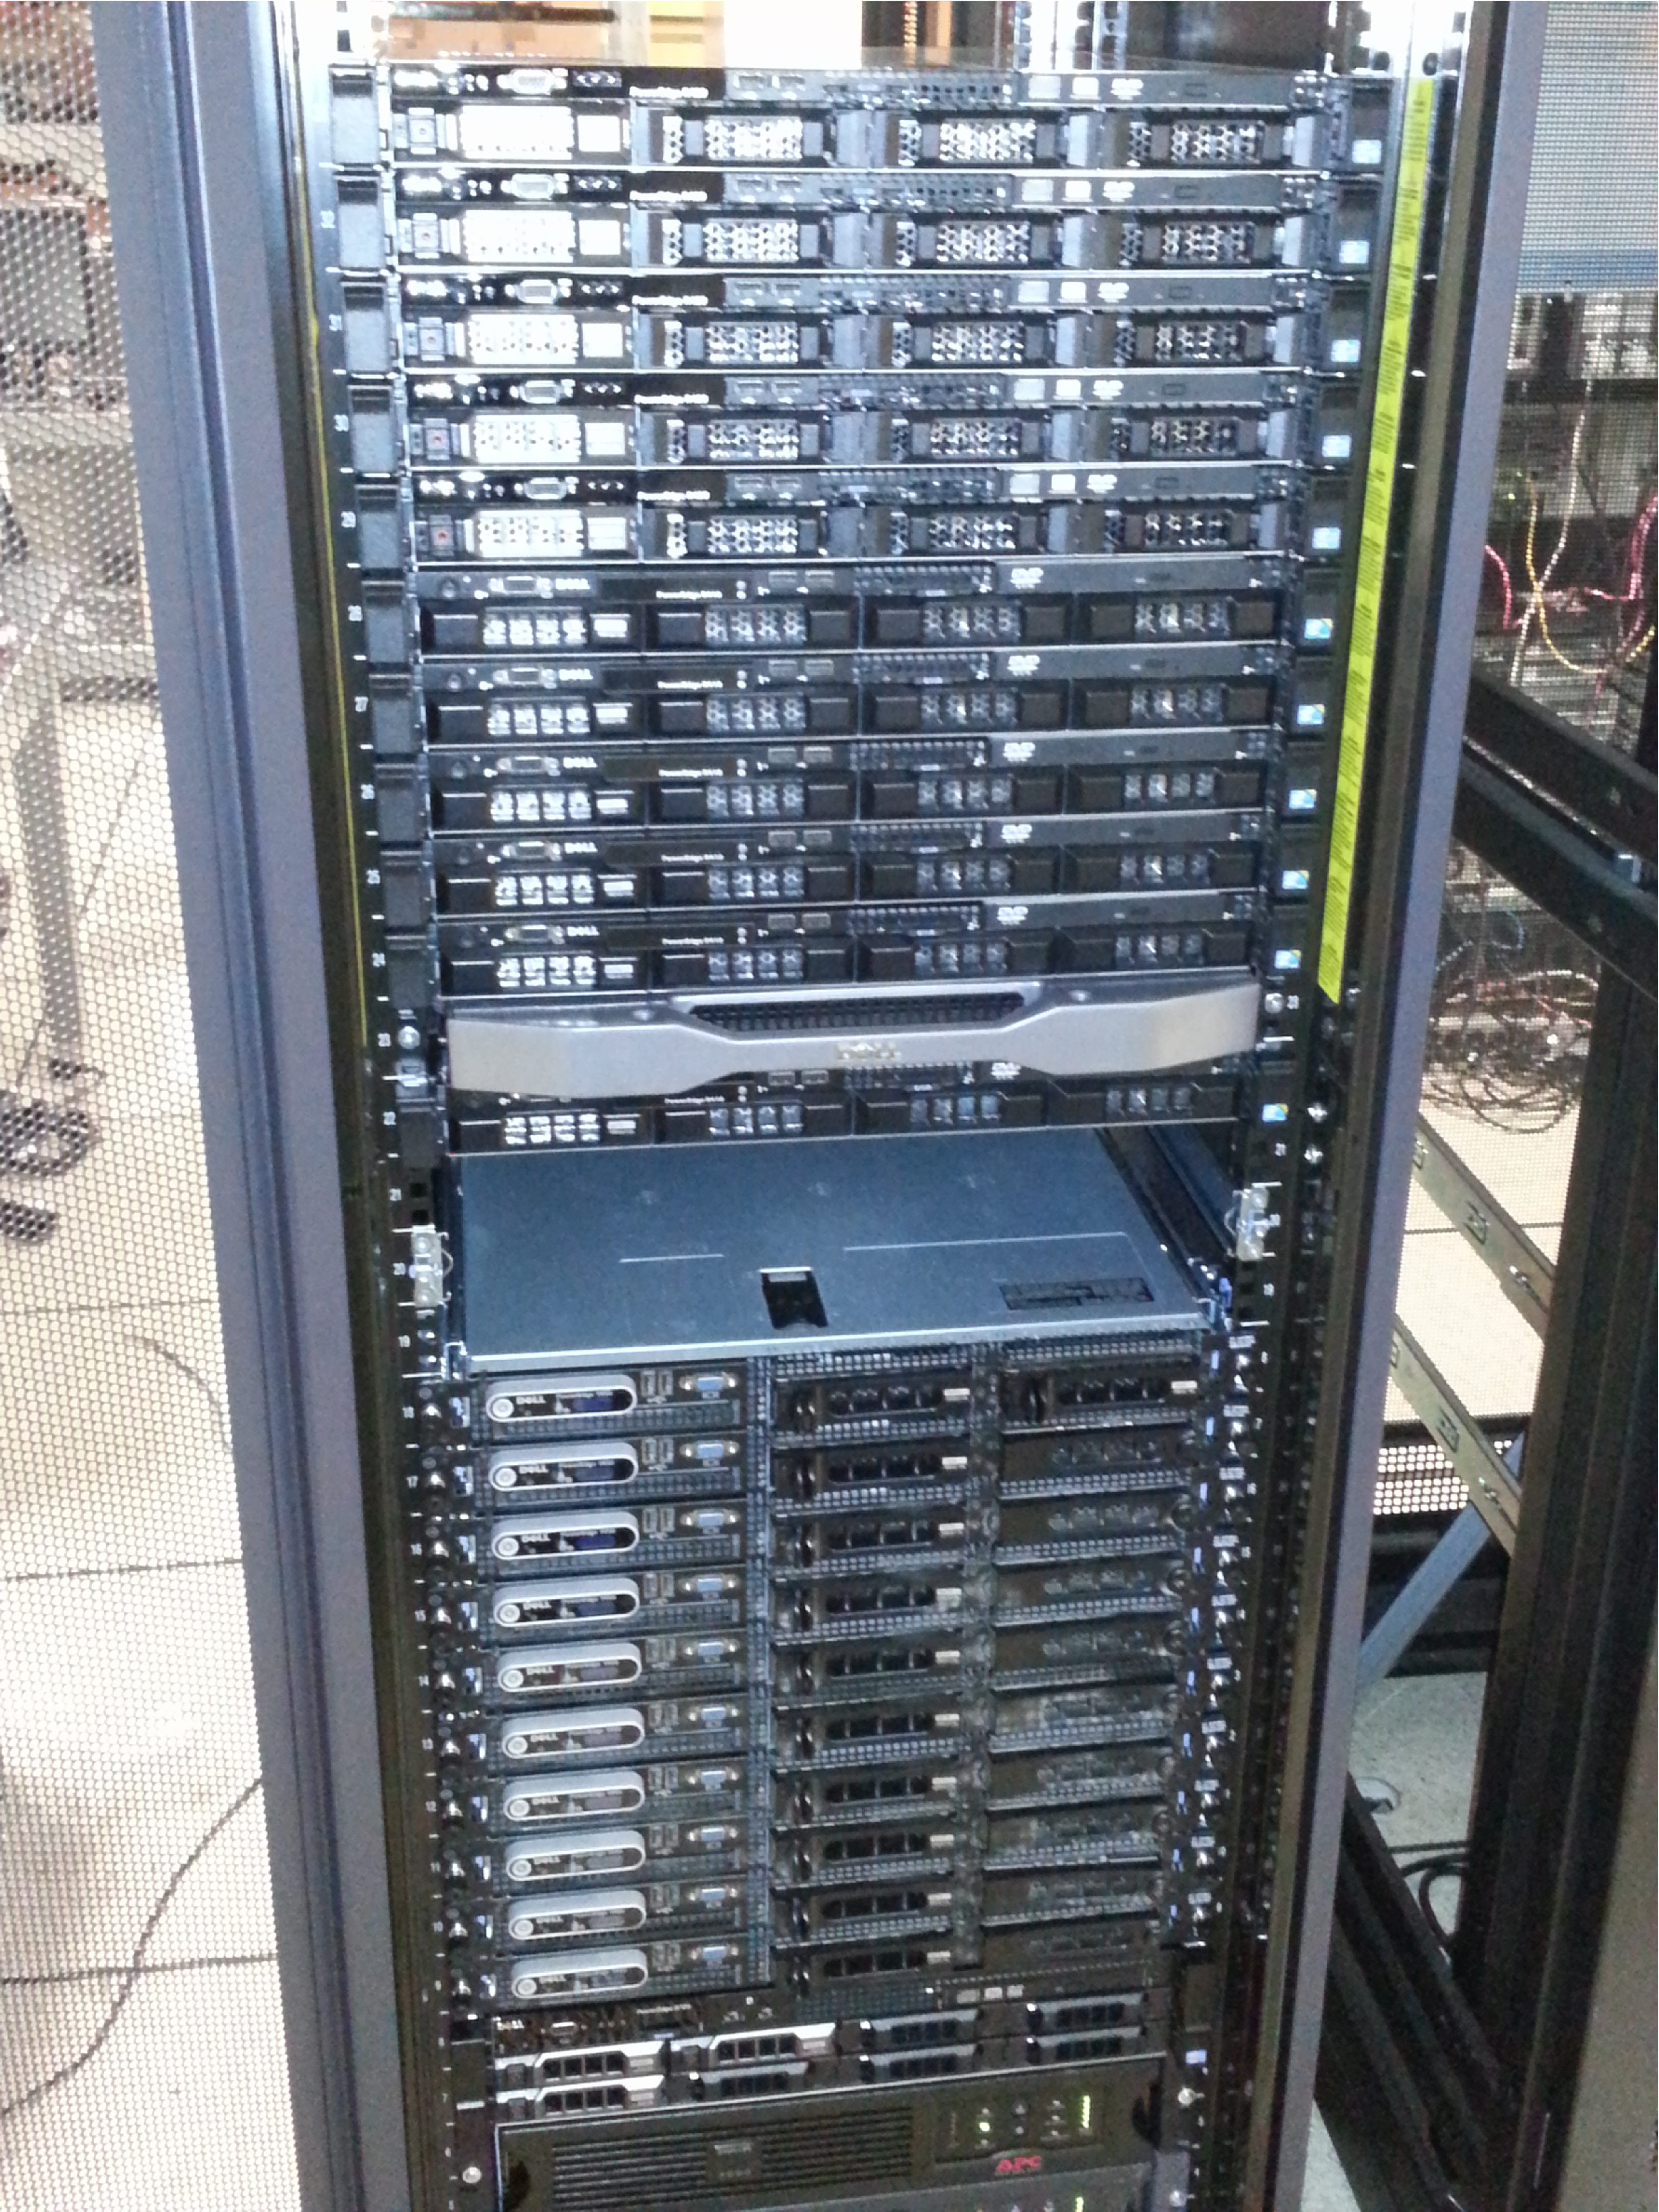
\includegraphics[width=.8\textwidth]{cluster}
  \end{figure}


\end{columns}

\end{frame}


\section{Creating a WCRL Communication Theory Cloud Account}
\begin{frame}
  \frametitle{Creating a WCTC Web Interface Account}

  \begin{itemize}

  \item An account is required to access the WCTC web interface.

  \item To create an account, access \url{http://wcrl.csee.wvu.edu/wctc} and follow the link ``Request Login''.

    \begin{figure}
      \centering
      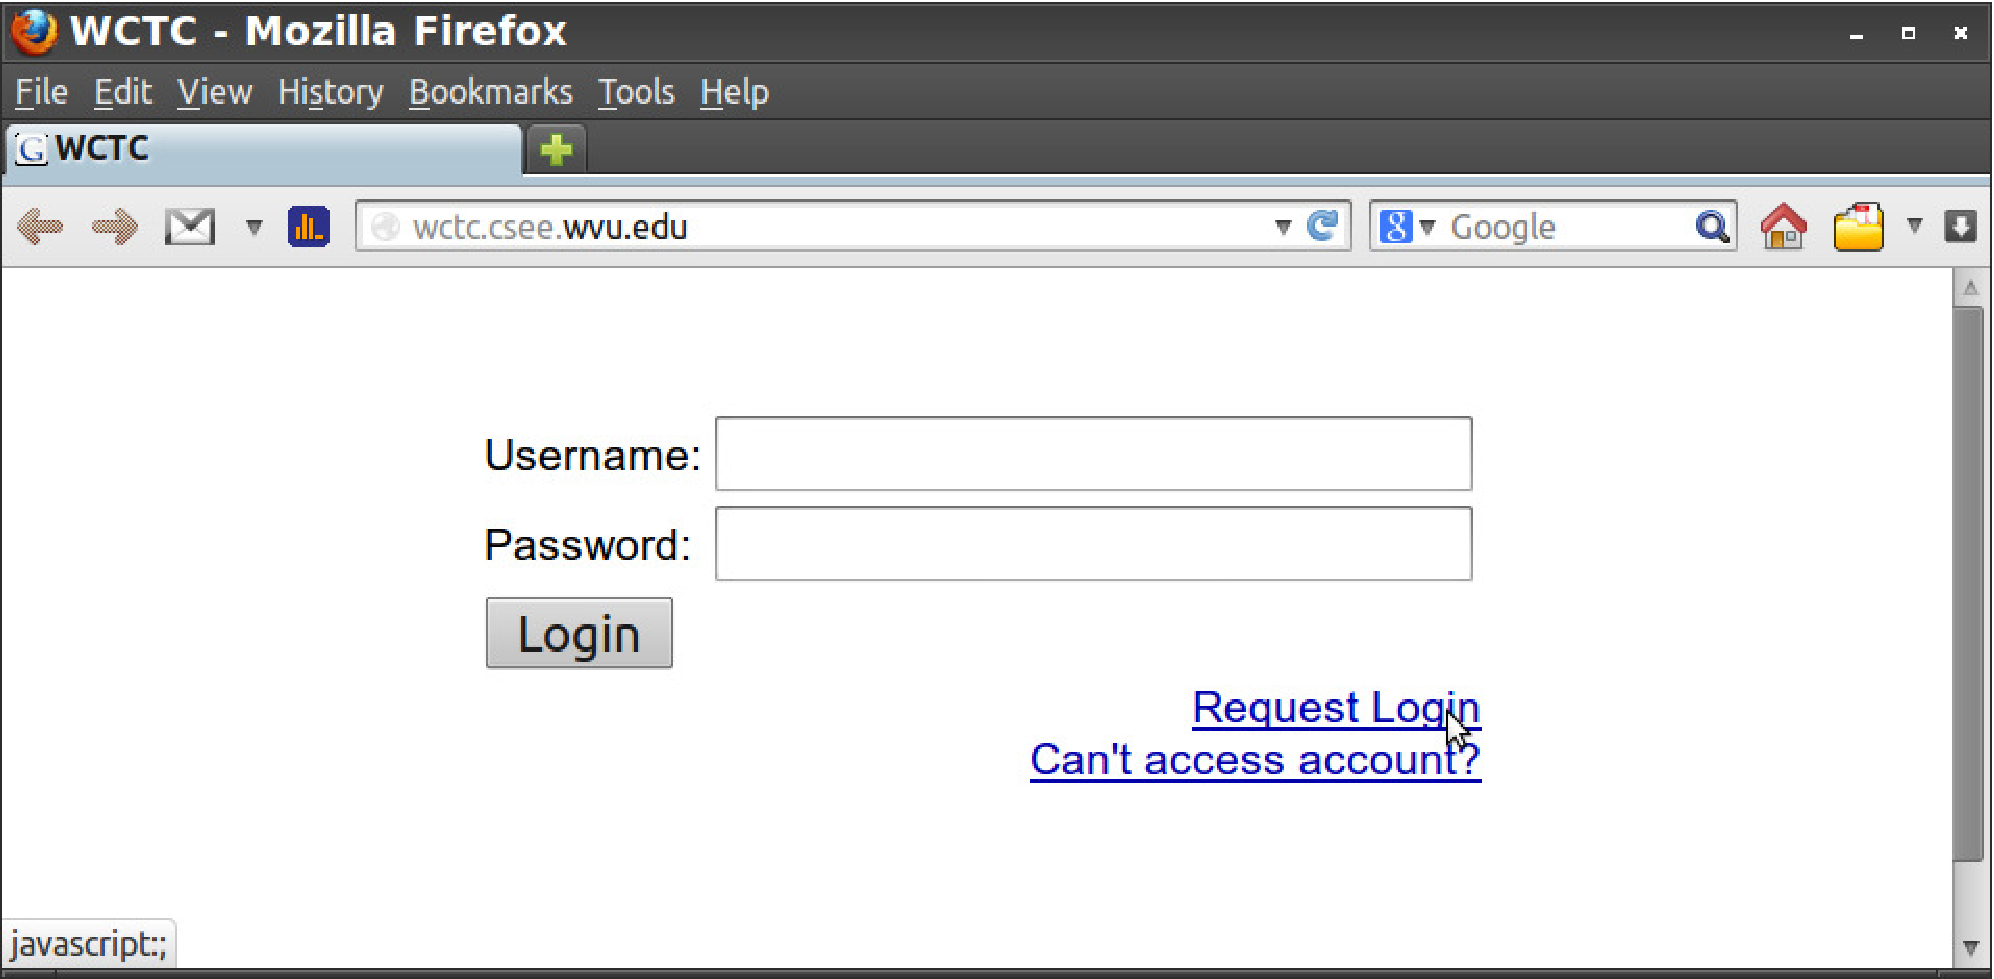
\includegraphics[width=.7\textwidth]{wcrlctc_account}
    \end{figure}

    \begin{itemize}
    \item{ You will receive an e-mail containing your username and password. }
    \end{itemize}

  \item Your WCTC account allows you to submit CML error-rate jobs for execution and download results.

  \end{itemize}

\end{frame}


\section{Job Submission Tutorial: BPSK in AWGN}

% webcml functionality
\begin{frame}
  \frametitle{Introduction}
\begin{itemize_loose}
\item The purpose of this tutorial is to introduce the user to submitting jobs to the WCTC web interface.

\item A CML error-rate simulation of BPSK modulation in an AWGN channel is submitted as a WCTC job.

\item The job results are saved to the user's local machine and plotted using CML.
\end{itemize_loose}

\end{frame}


\begin{frame}
\frametitle{Assumptions}
In this tutorial, it is assumed that the user has
\begin{itemize_loose}
\item A working MATLAB version $\geq$ 7.6 (R2008a)
\item Downloaded the WCRL Coded Modulation Library (CML) from \url{http://code.google.com/p/iscml/wiki/cml}.
\item Installed CML into local directory $<$CMLROOT$>$.
\item Followed the quickstart tutorial on the download site to familiarize with fundamental CML concepts.
\item Created a WCTC Web Interface Account as described in Section 3.
\end{itemize_loose}

\end{frame}

% tutorial terminology
\begin{frame}
\frametitle{Terminology}
The following terminology will be used throughout the tutorial:
\begin{itemize_loose}
\item Local computer - The user's computer running CML.
\item $<$CMLROOT$>$ - Directory on user's local computer containing CML.
\item Cluster - The server infrastructure administered by WCRL which hosts WCTC.
\item Job File - File generated by CML which contains the parameters of a single simulation for submission to using the WCTC web interface.
\end{itemize_loose}
\end{frame}


% starting cml
\begin{frame}
  \frametitle{ Starting CML }

  \begin{itemize}
  \item Start MATLAB and cd to $<$CMLROOT$>$.
  \item Execute function CmlStartup() to initialize CML.
  \end{itemize}

  \begin{figure}
    \centering
    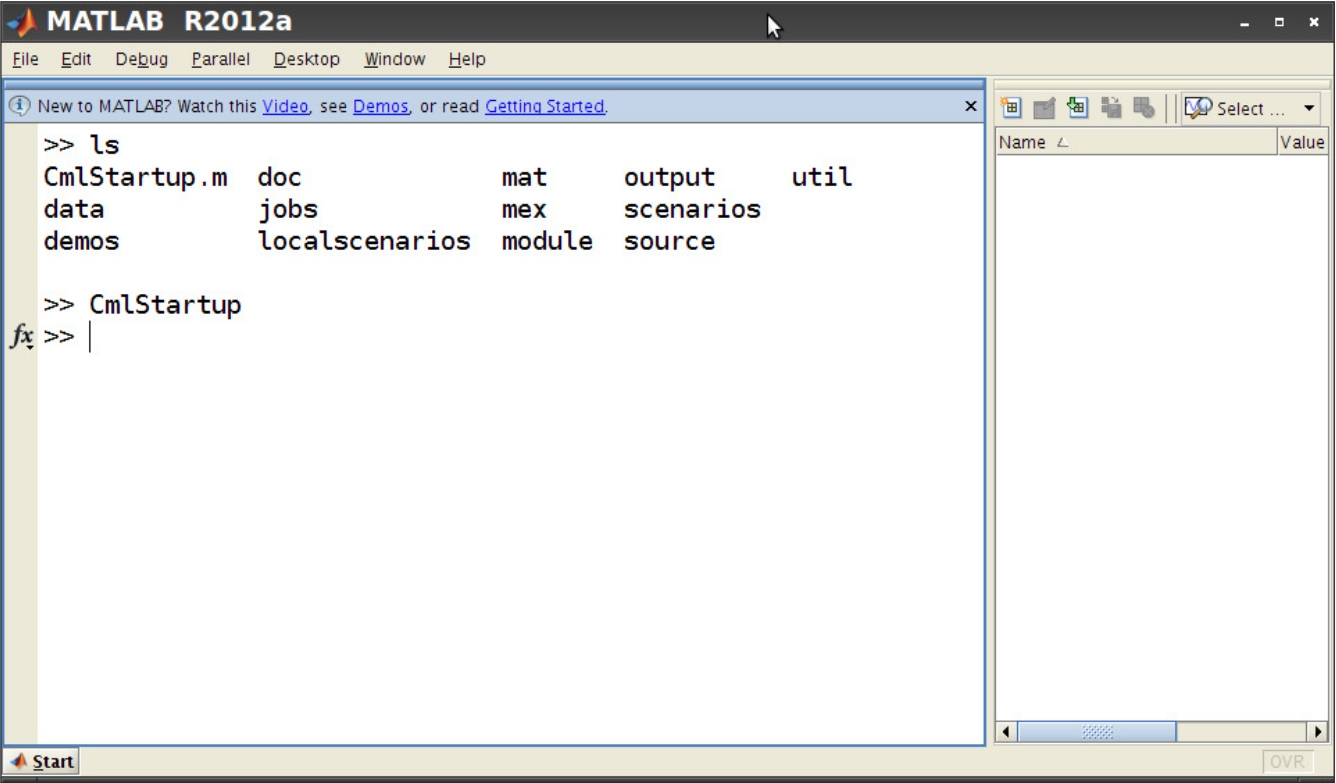
\includegraphics[width=.8\textwidth]{cml_startup}
  \end{figure}

\end{frame}




% creating a job file
\begin{frame}
  \frametitle{ Creating a Job File }

  In this example, we create a job file for an error-rate simulation of uncoded BPSK in AWGN.
  \begin{itemize}
  \item Scenario: UncodedScenarios
  \item Record: 1
  \end{itemize}

  \begin{figure}
    \centering
    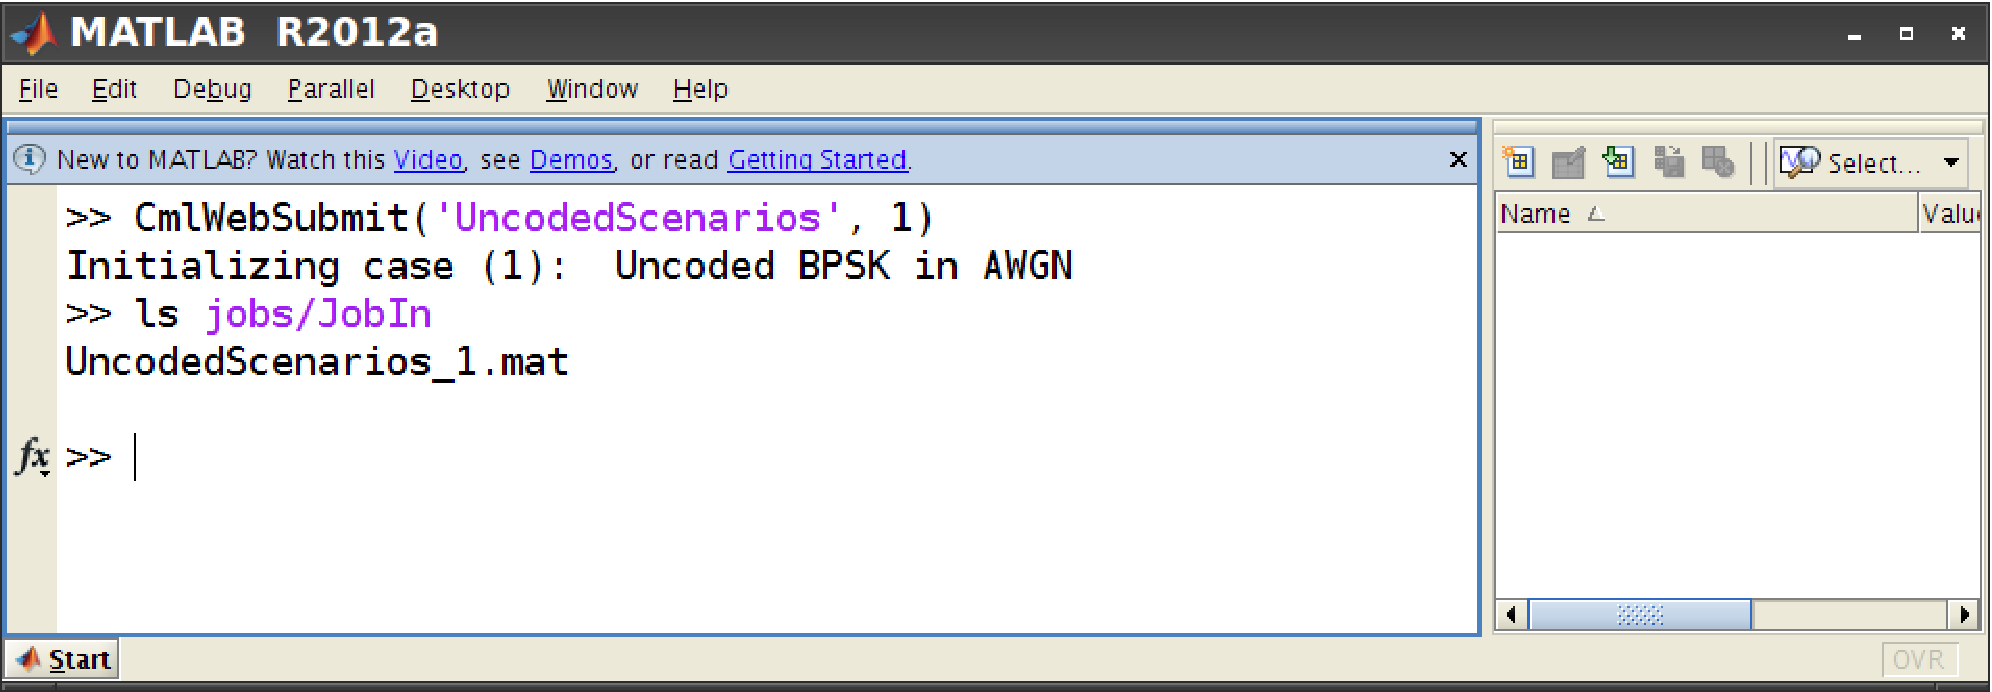
\includegraphics[width=.8\textwidth]{cml_websubmit}
  \end{figure}

  \begin{itemize}
  \item CmlWebSubmit() has created the job file $<$CMLROOT$>$/jobs/JobIn/UncodedScenarios\_1.mat
  \end{itemize}

\end{frame}




% web interface login
\begin{frame}
  \frametitle{WCTC Web Interface Login}

  \begin{itemize_loose}
  \item To submit the generated job file, log in to the WCTC web interface located at
    \\ \url{http://wctc.csee.wvu.edu}
  \item Use the credentials created in Section 2.
  \end{itemize_loose}

  \centering
  \begin{figure}
    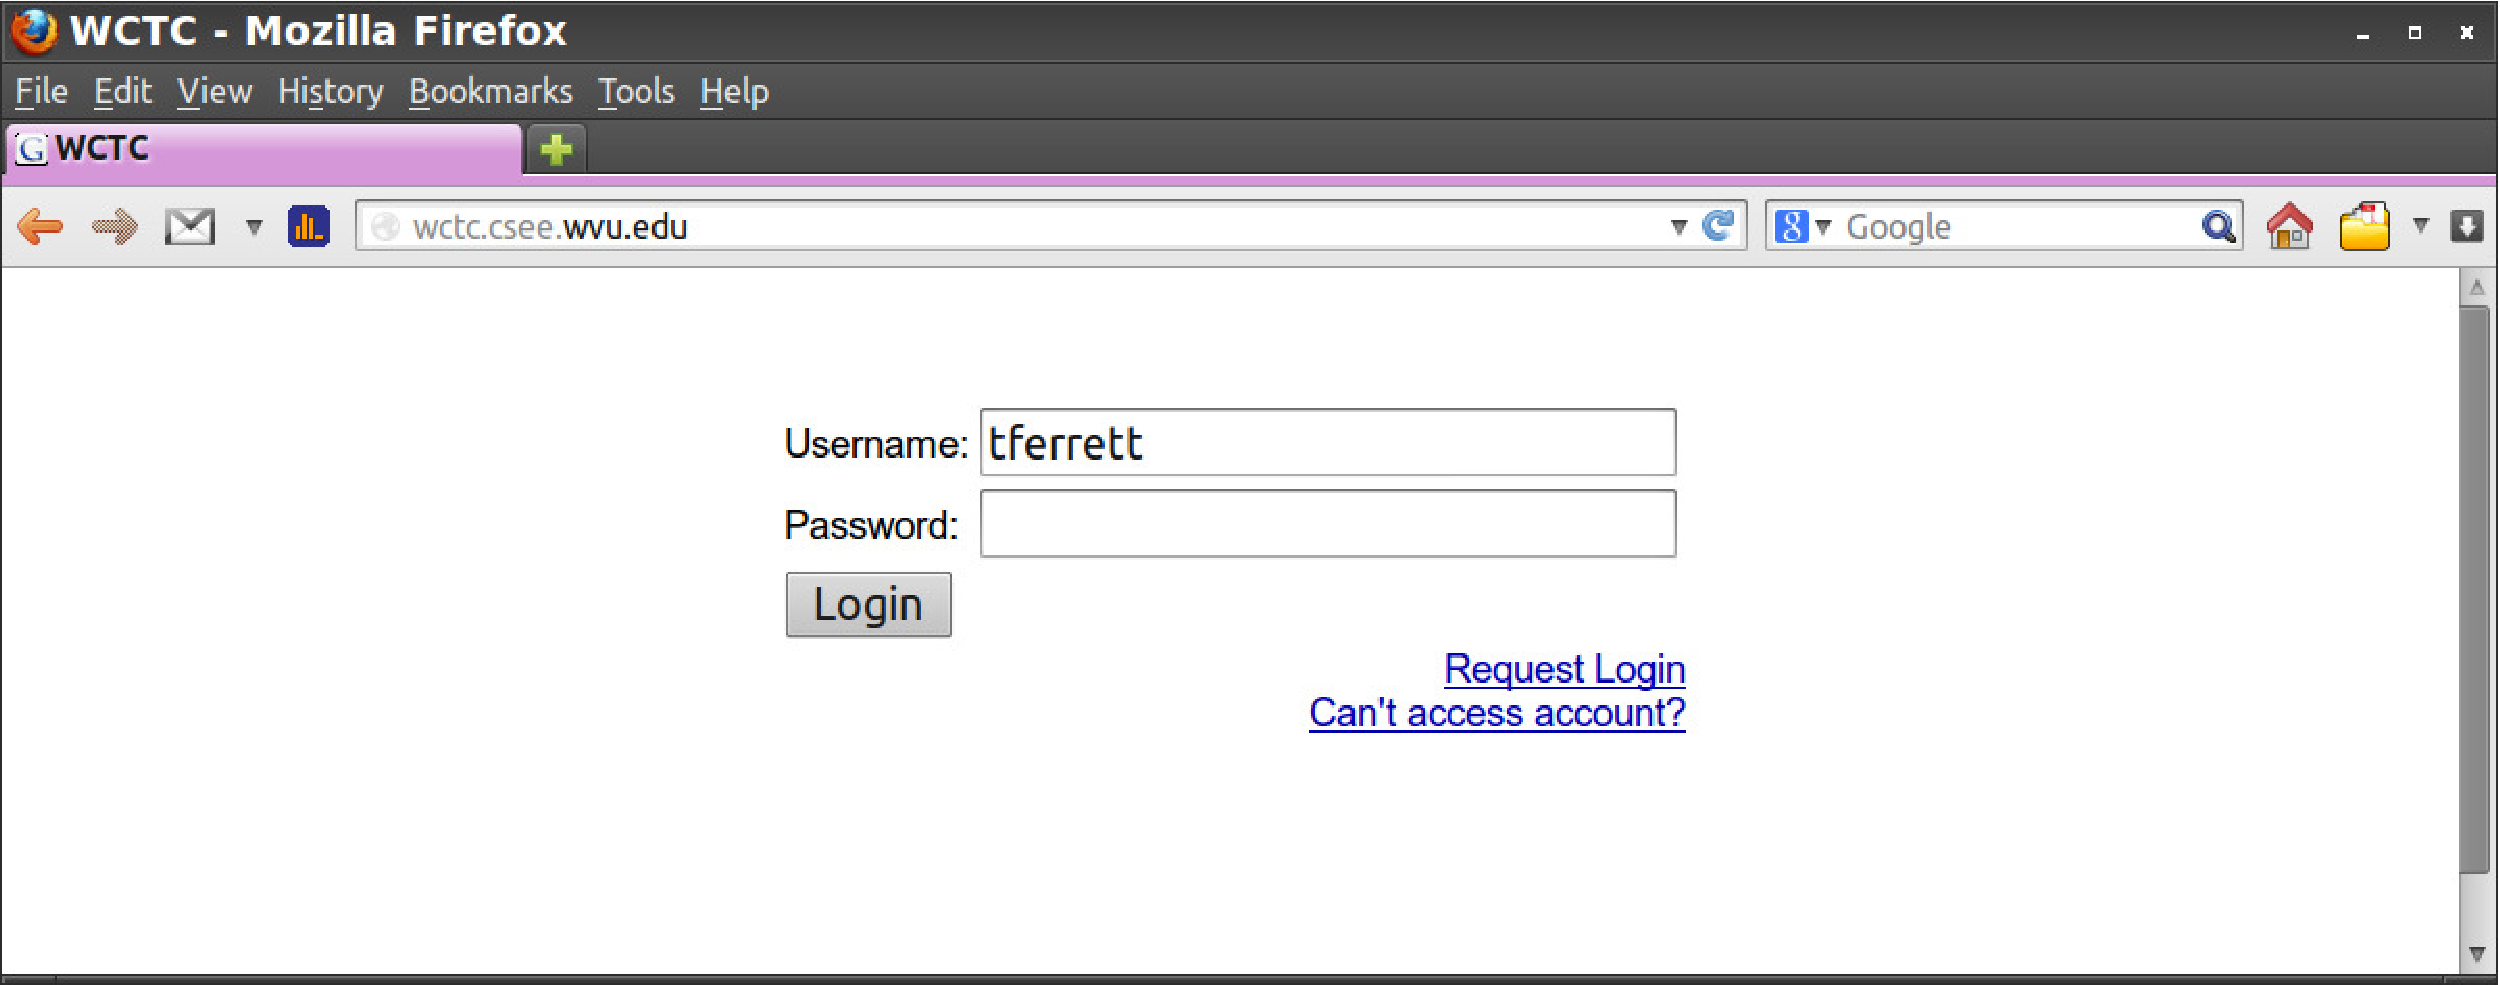
\includegraphics[width=0.9\textwidth]{wcrlctc_login}
  \end{figure}

\end{frame}




% job file submission
\begin{frame}
  \frametitle{Job File Submission}

  In this step we will add the job file to the input queue for execution.
  \begin{itemize}
  \item Click the tab ``My Jobs'', bringing up the job manipulation interface.
  \item In the drop-down next to the button ``Add Job'', select project ``cml''.
  \item Click the button ``Add Job'' as shown in the figure.
  \end{itemize}

  \centering

  \begin{figure}
    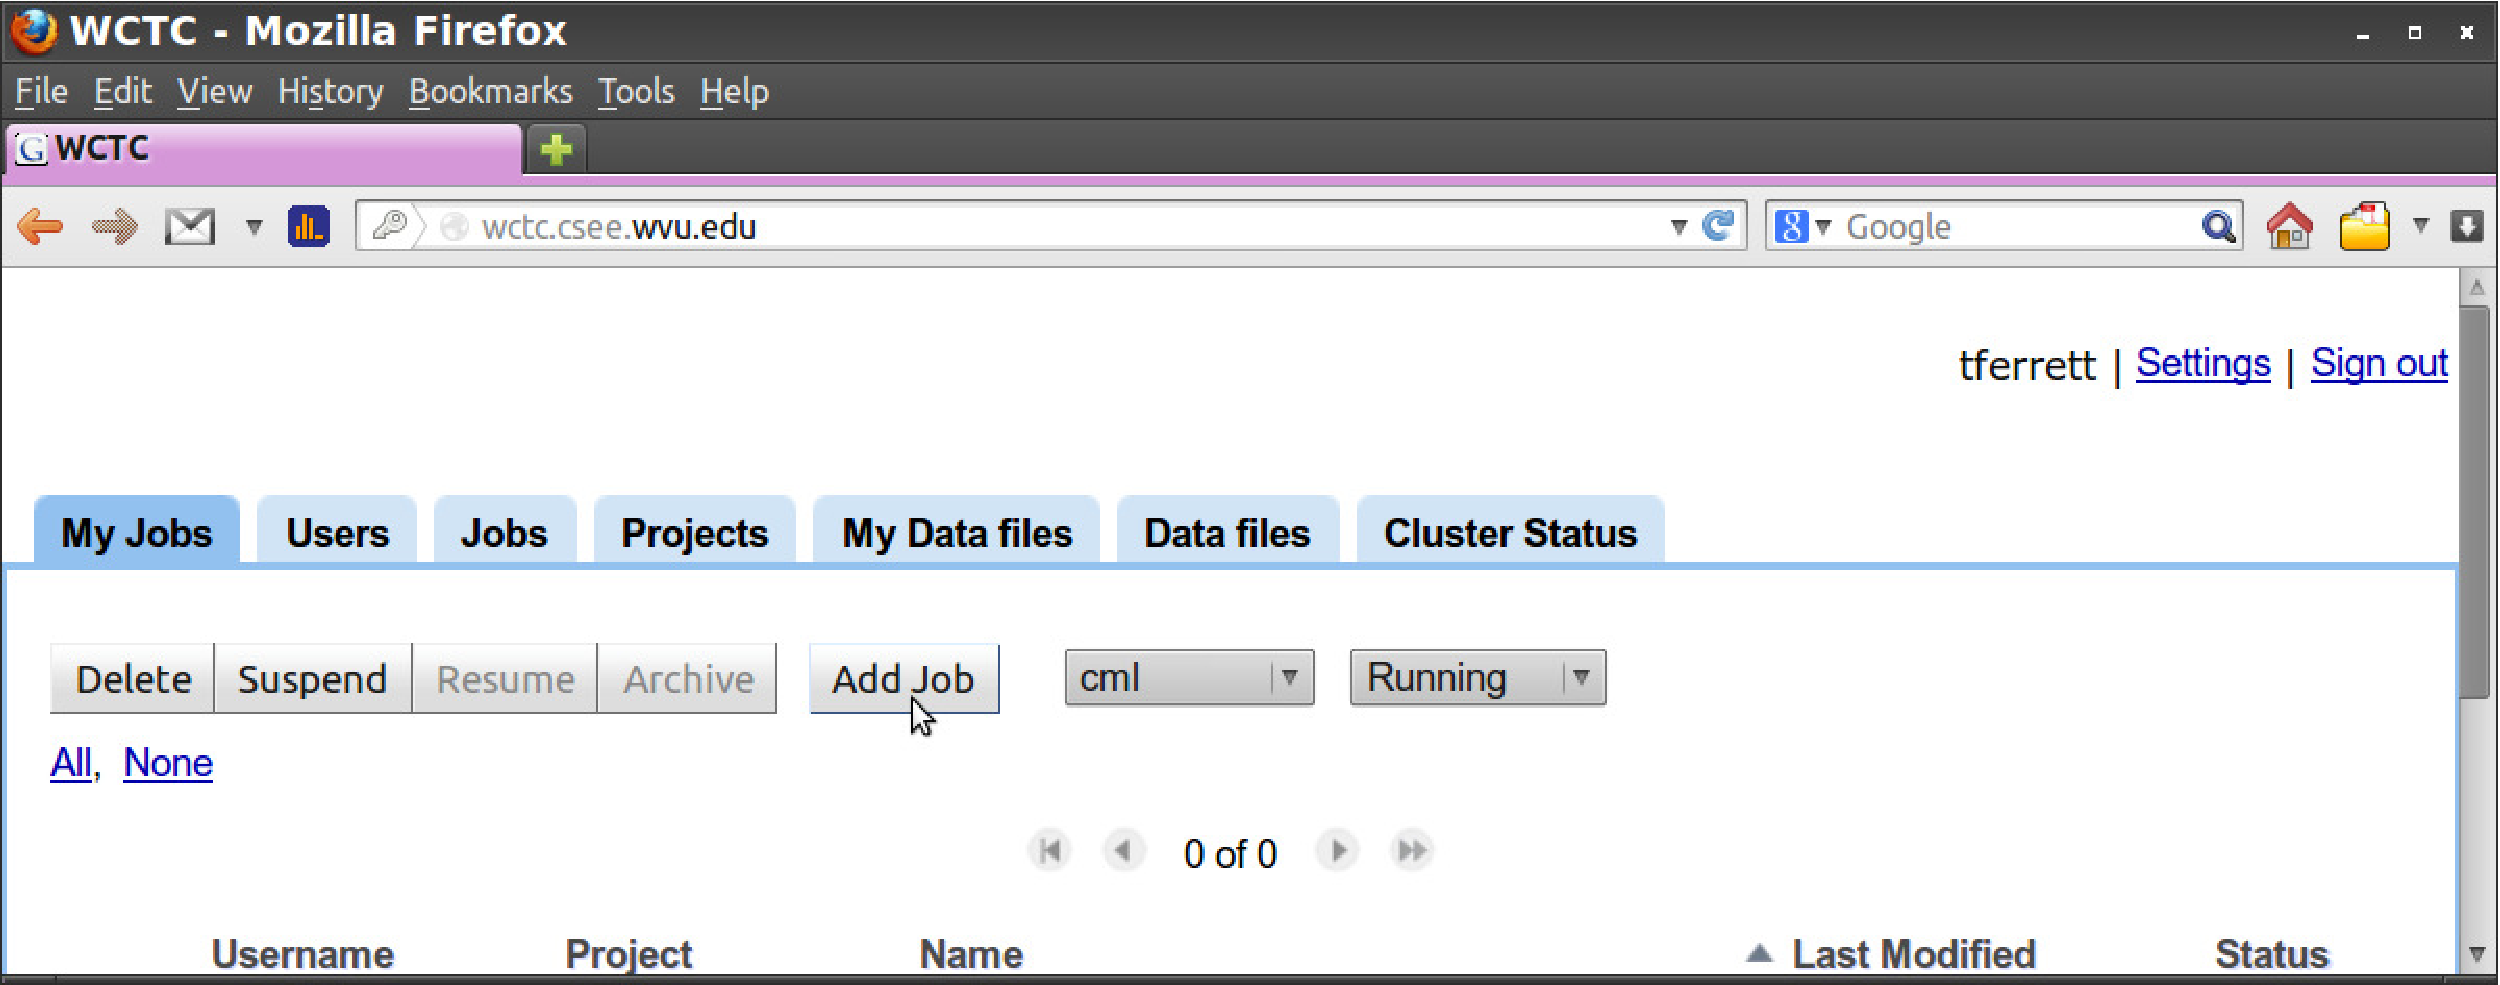
\includegraphics[width=0.9\textwidth]{wcrlctc_addjob}
  \end{figure}

\end{frame}




% file submission interface
\begin{frame}

  Select the job file to upload from the local filesystem.
  \begin{itemize}
  \item Click the ``Browse'' button. This will open a file selection dialog.
  \item Select the job file $<$CMLROOT$>$/jobs/JobIn/UncodedScenarios\_1.mat
  \end{itemize}

  \centering
  \begin{figure}
    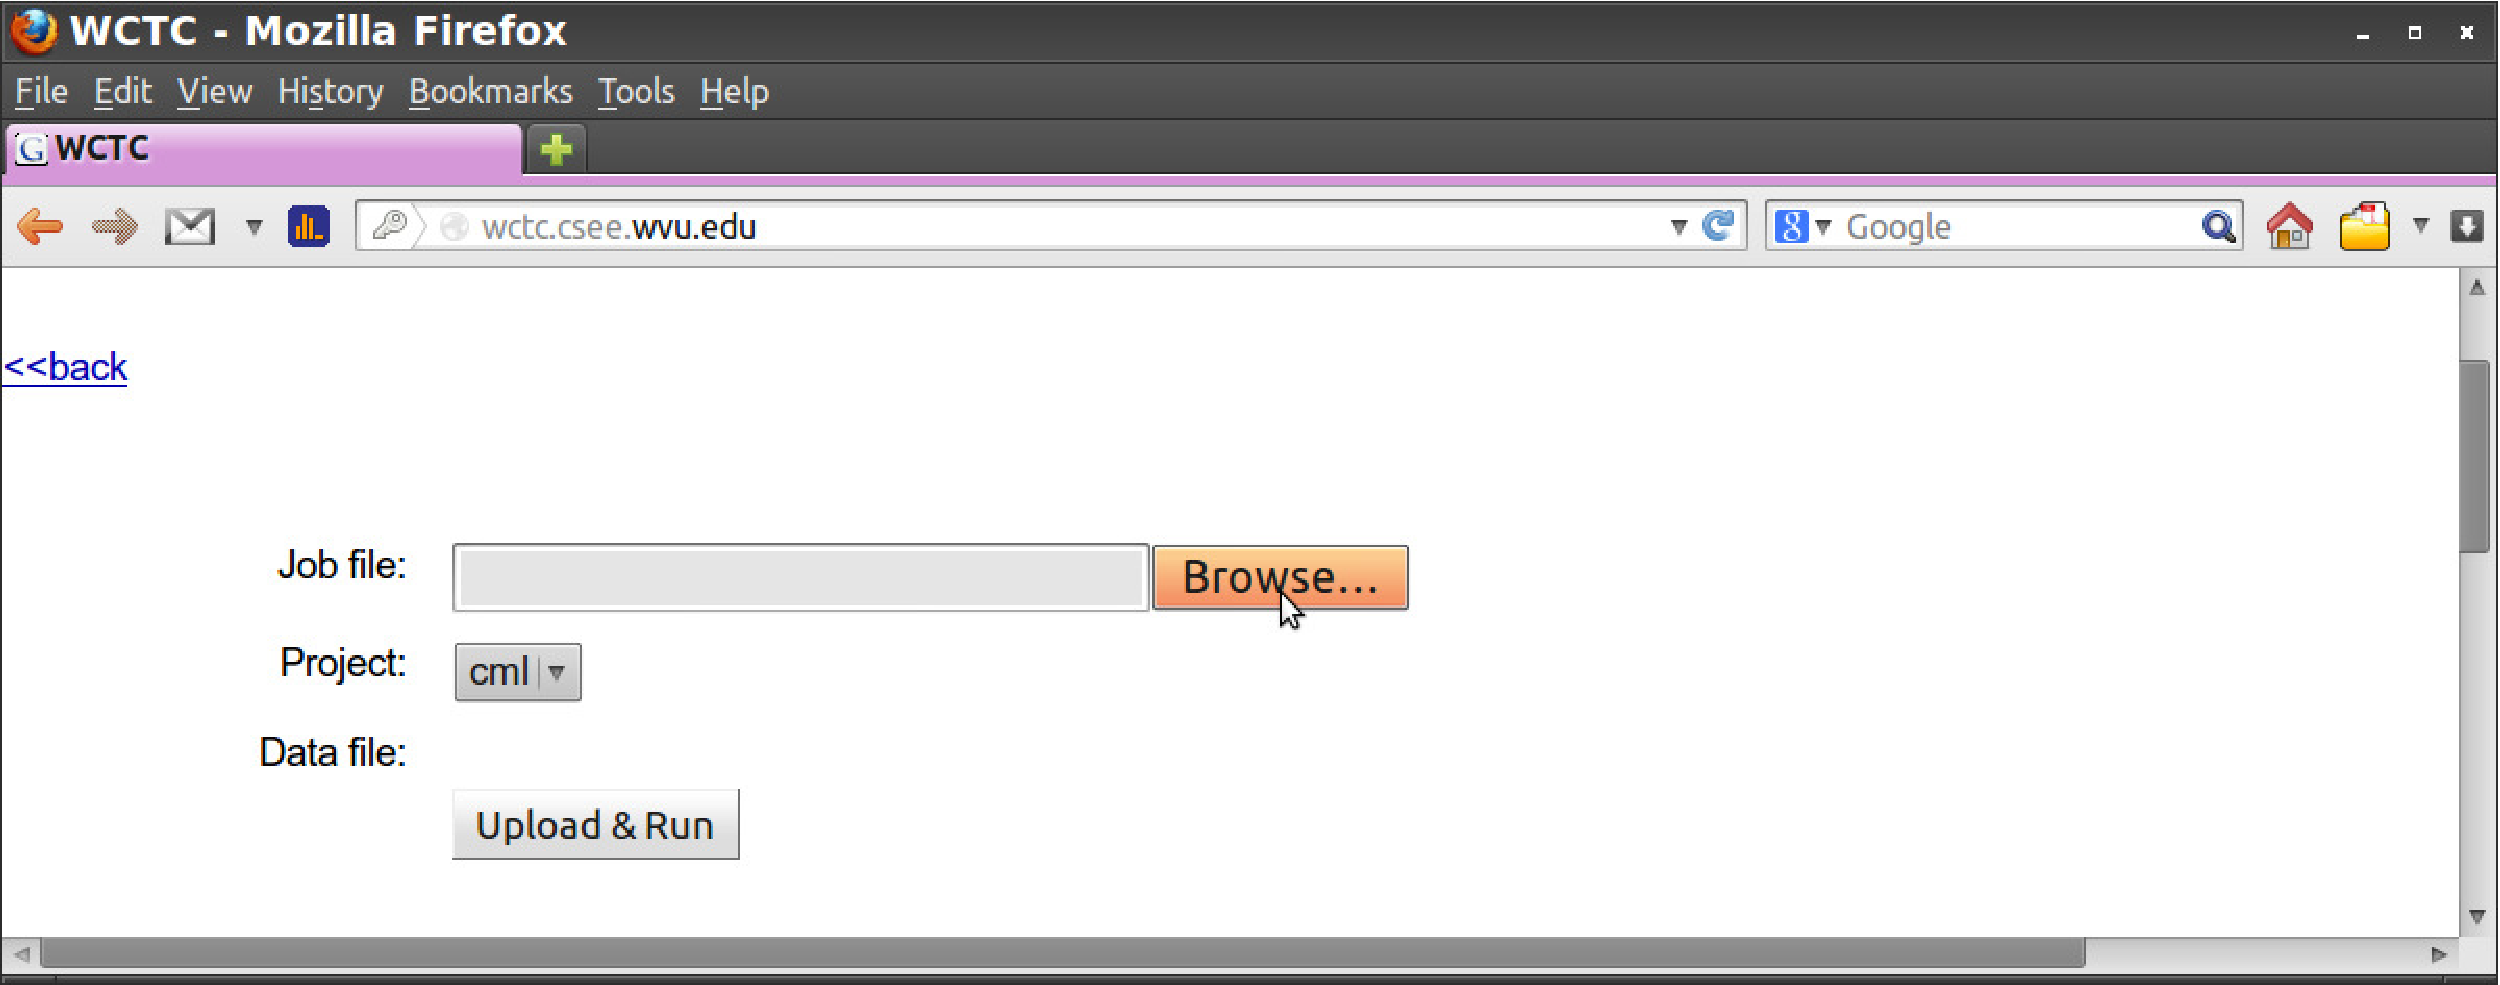
\includegraphics[width=0.7\textwidth]{wcrlctc_browsejob}
  \end{figure}

  \vspace{-8mm}

  \begin{figure}
    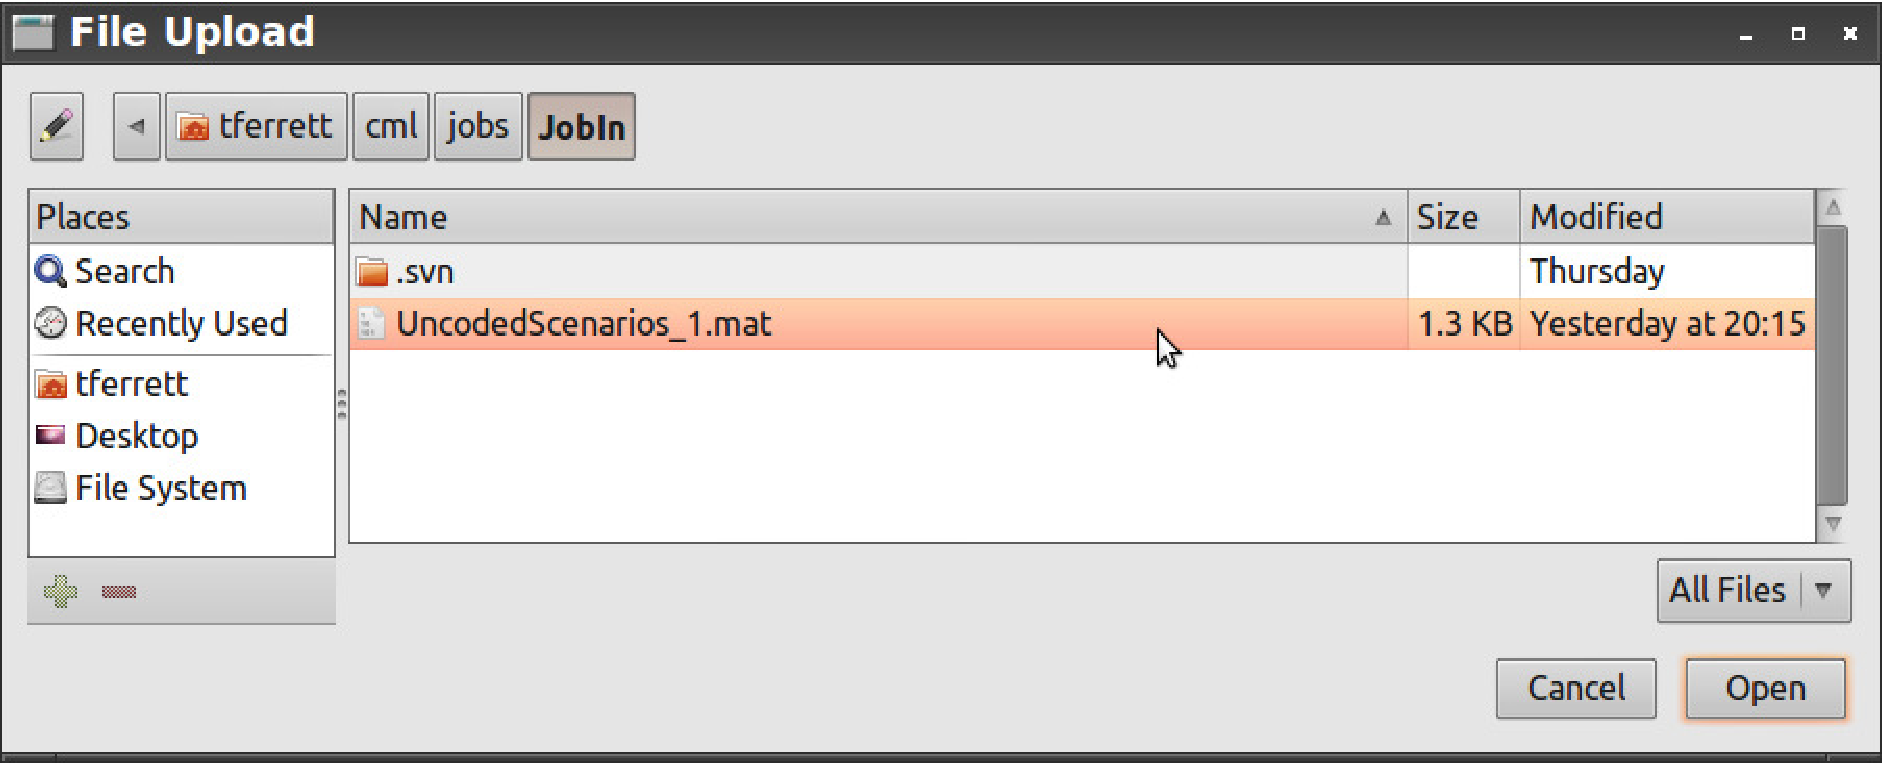
\includegraphics[width=0.7\textwidth]{wcrlctc_jobfile}
  \end{figure}

\end{frame}




% upload and run
\begin{frame}

  Uploading and running the job file submits the job to the cluster input queue for execution.
  \begin{itemize}
  \item Click ``Upload $\&$ Run'' to submit the job to the input queue.
  \end{itemize}

  \centering
  \begin{figure}
    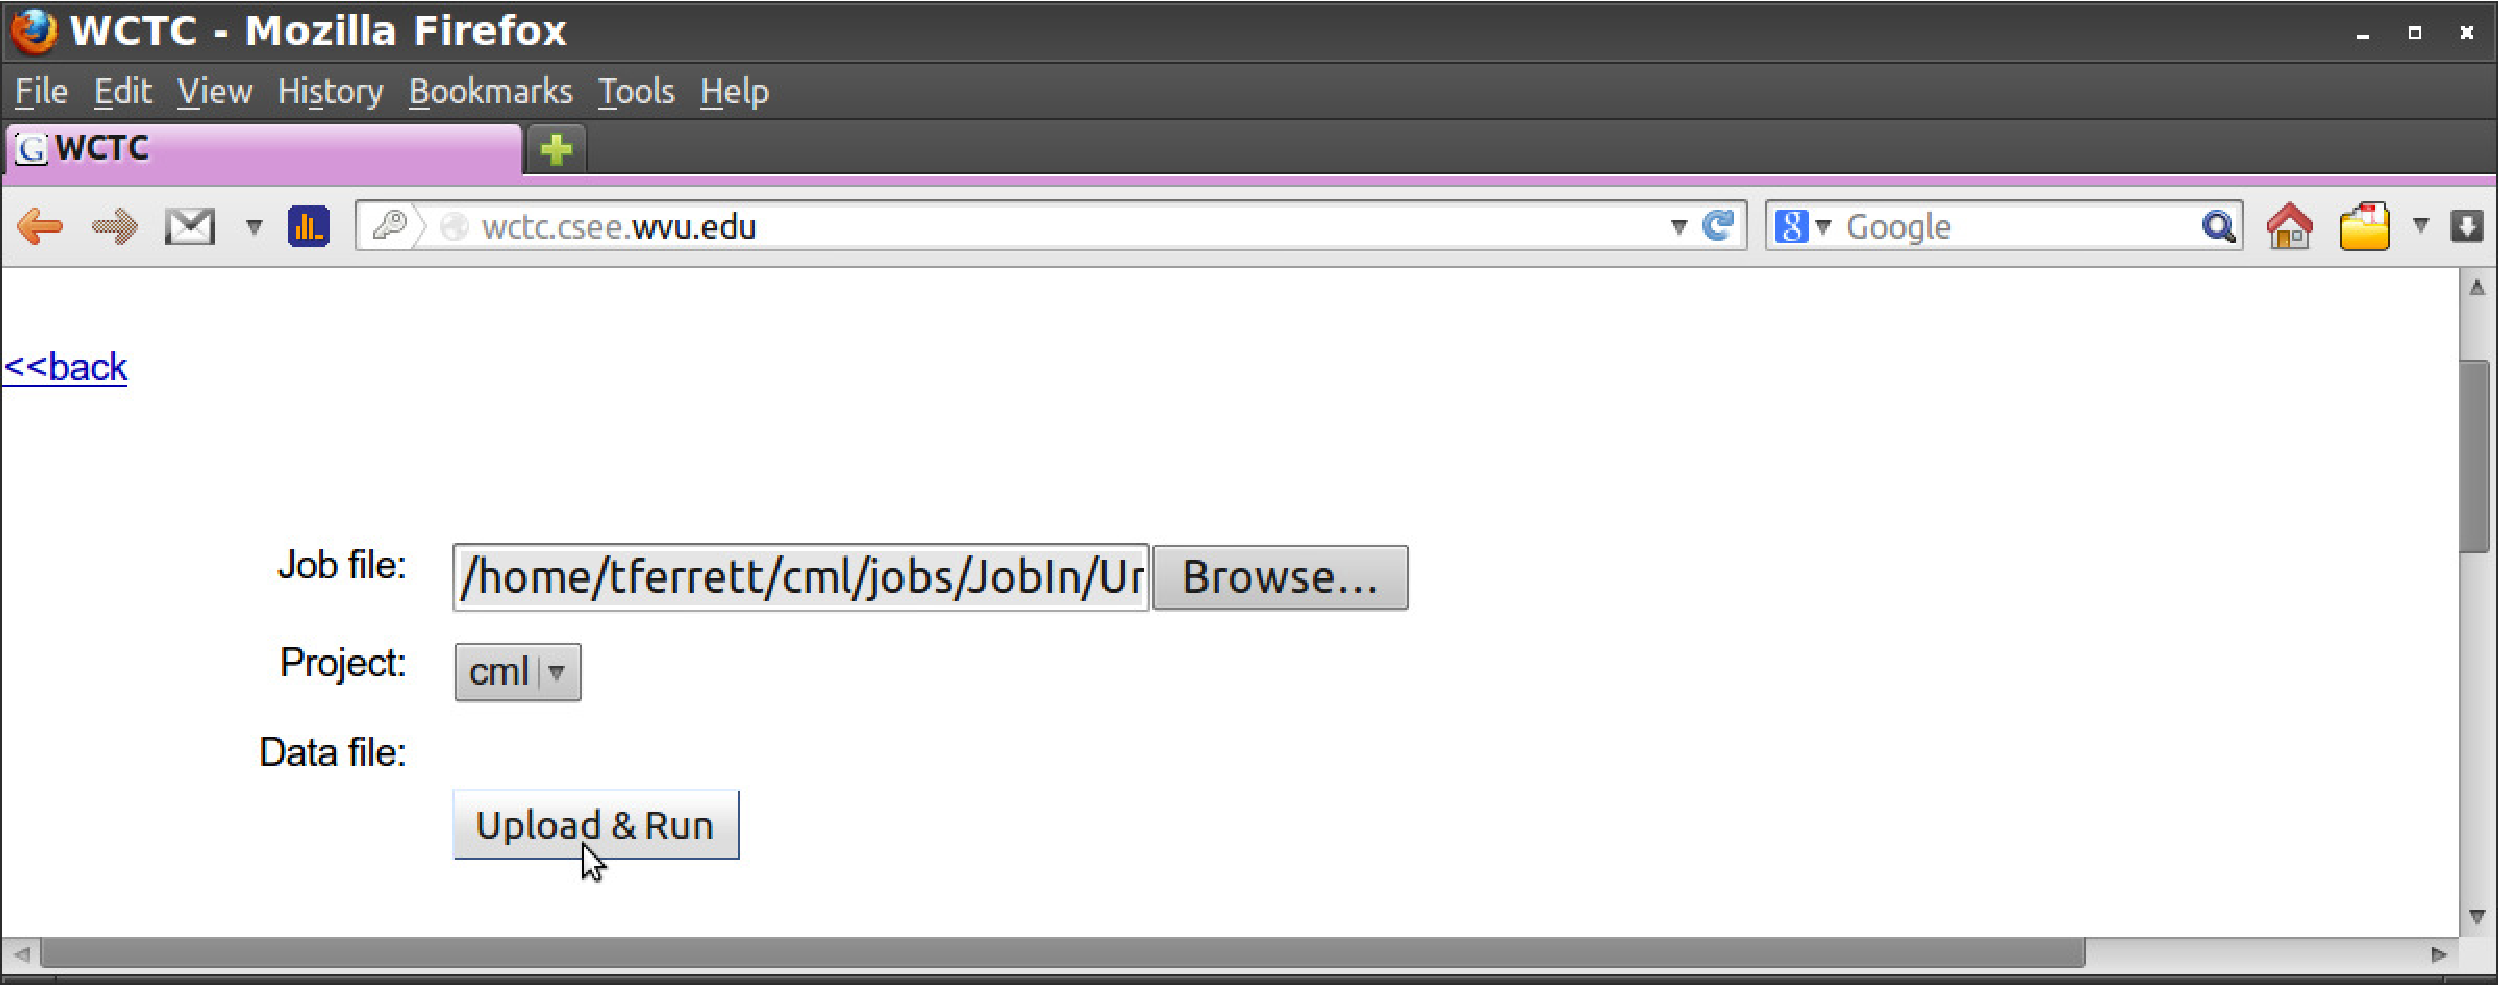
\includegraphics[width=0.9\textwidth]{wcrlctc_upload}
  \end{figure}

\end{frame}




% job execution
\begin{frame}
  \frametitle{Job Execution}

  The job is now executed on the cluster when resources are available.\\
  To check for job completion,

  \begin{itemize}
  \item In the drop-down menu highlighted in the figure, select ``Done''.  
  \item The completed job will appear in the table at the bottom of the page, as shown in the figure.
  \end{itemize}

  \begin{figure}
    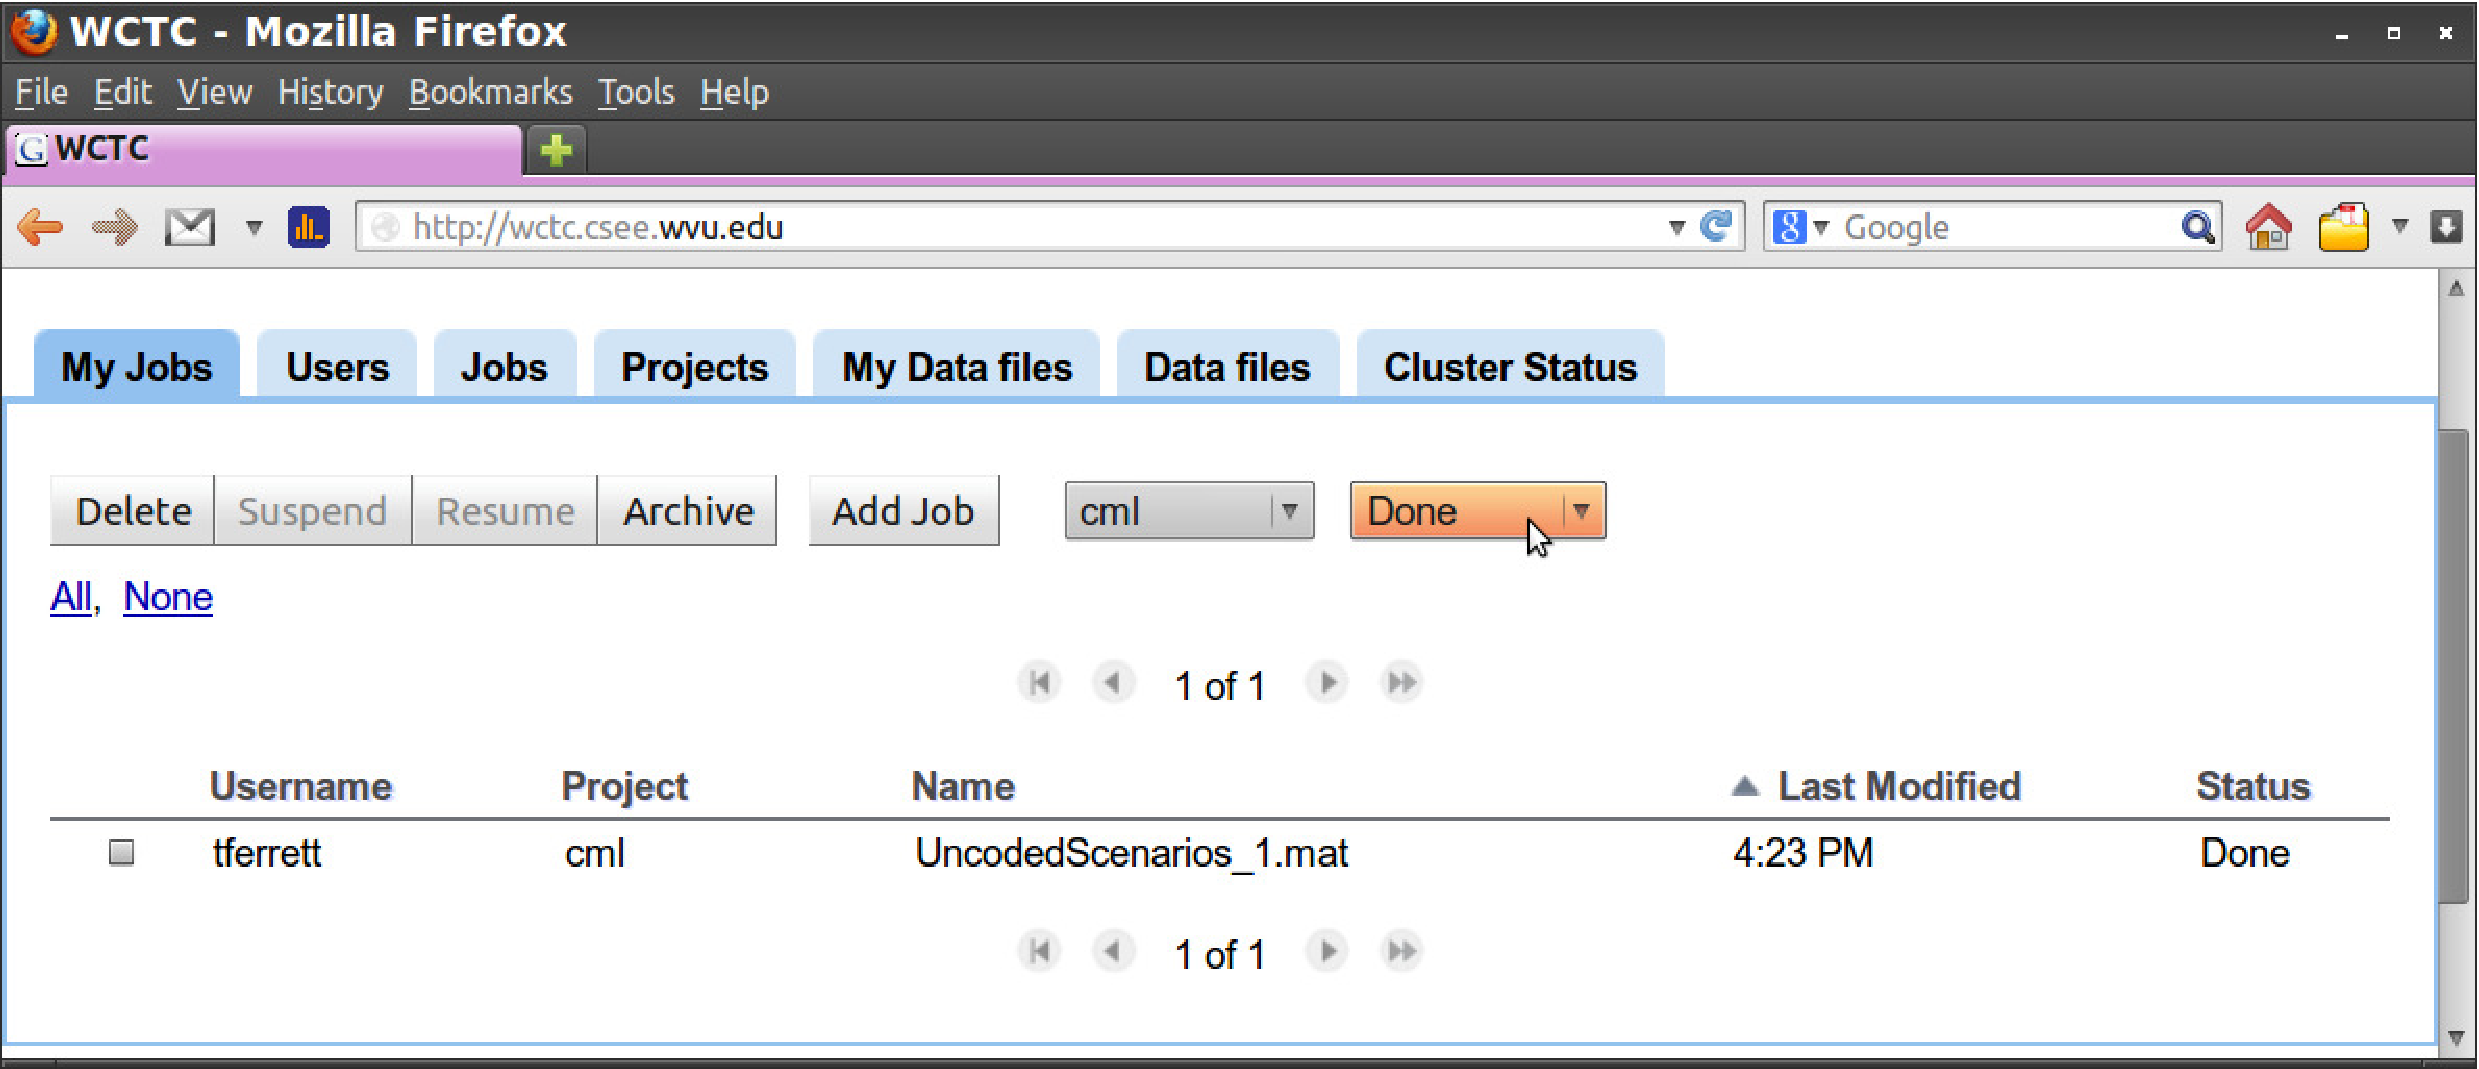
\includegraphics[width=0.9\textwidth]{wcrlctc_done}
  \end{figure}

\end{frame}




% results retrieval
\begin{frame}
  \frametitle{Job Results Retrieval}

  Now that the job is complete, retrieve the results for local plotting.
  \begin{itemize}
  \item Click the link to the name of the job file as shown in the figure and perform a ``Save As'' operation.
  \end{itemize}

  \centering
  \begin{figure}
    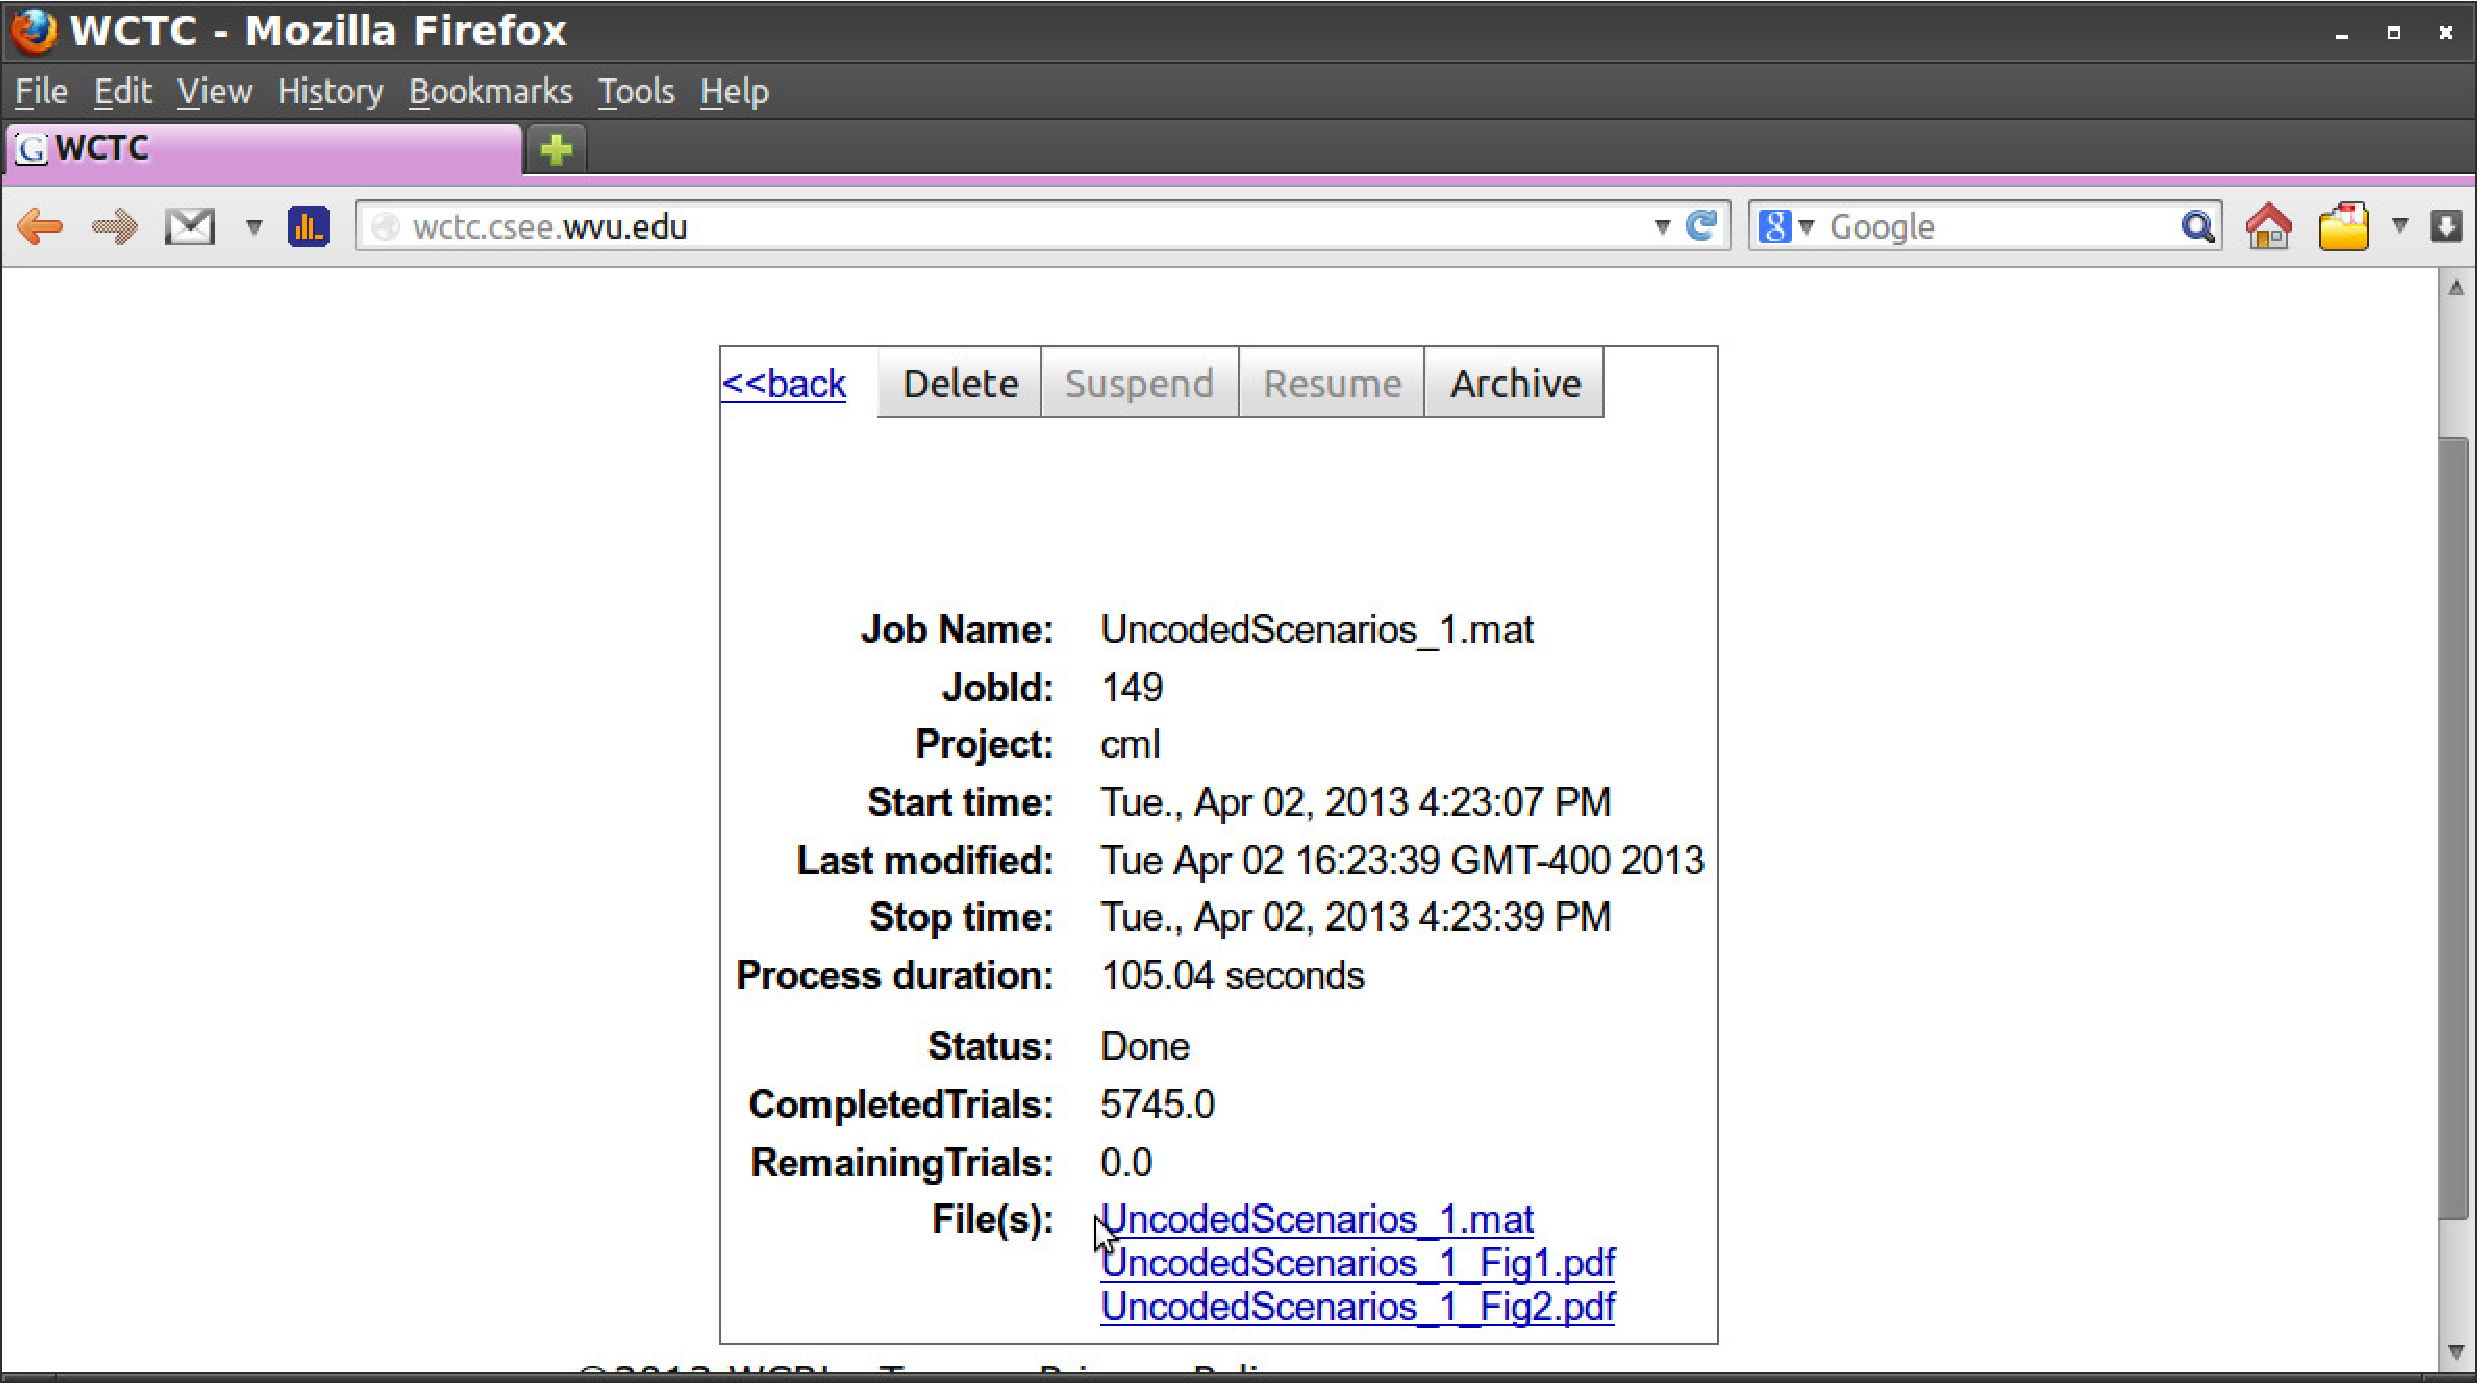
\includegraphics[width=0.9\textwidth]{wcrlctc_downjob}
  \end{figure}

\end{frame}




% saving to jobout
\begin{frame}

  \begin{itemize_loose}
  \item All completed jobs must be placed in $<$CMLROOT$>$/jobs/JobOut for processing
    by CML.
  \item When prompted for a location to save the completed job file, specify
    \begin{itemize}
    \item $<$CMLROOT$>$/jobs/JobOut/UncodedScenarios\_1.mat
    \end{itemize}
    as shown in the figure.
  \end{itemize_loose}

  \centering
  \begin{figure}
    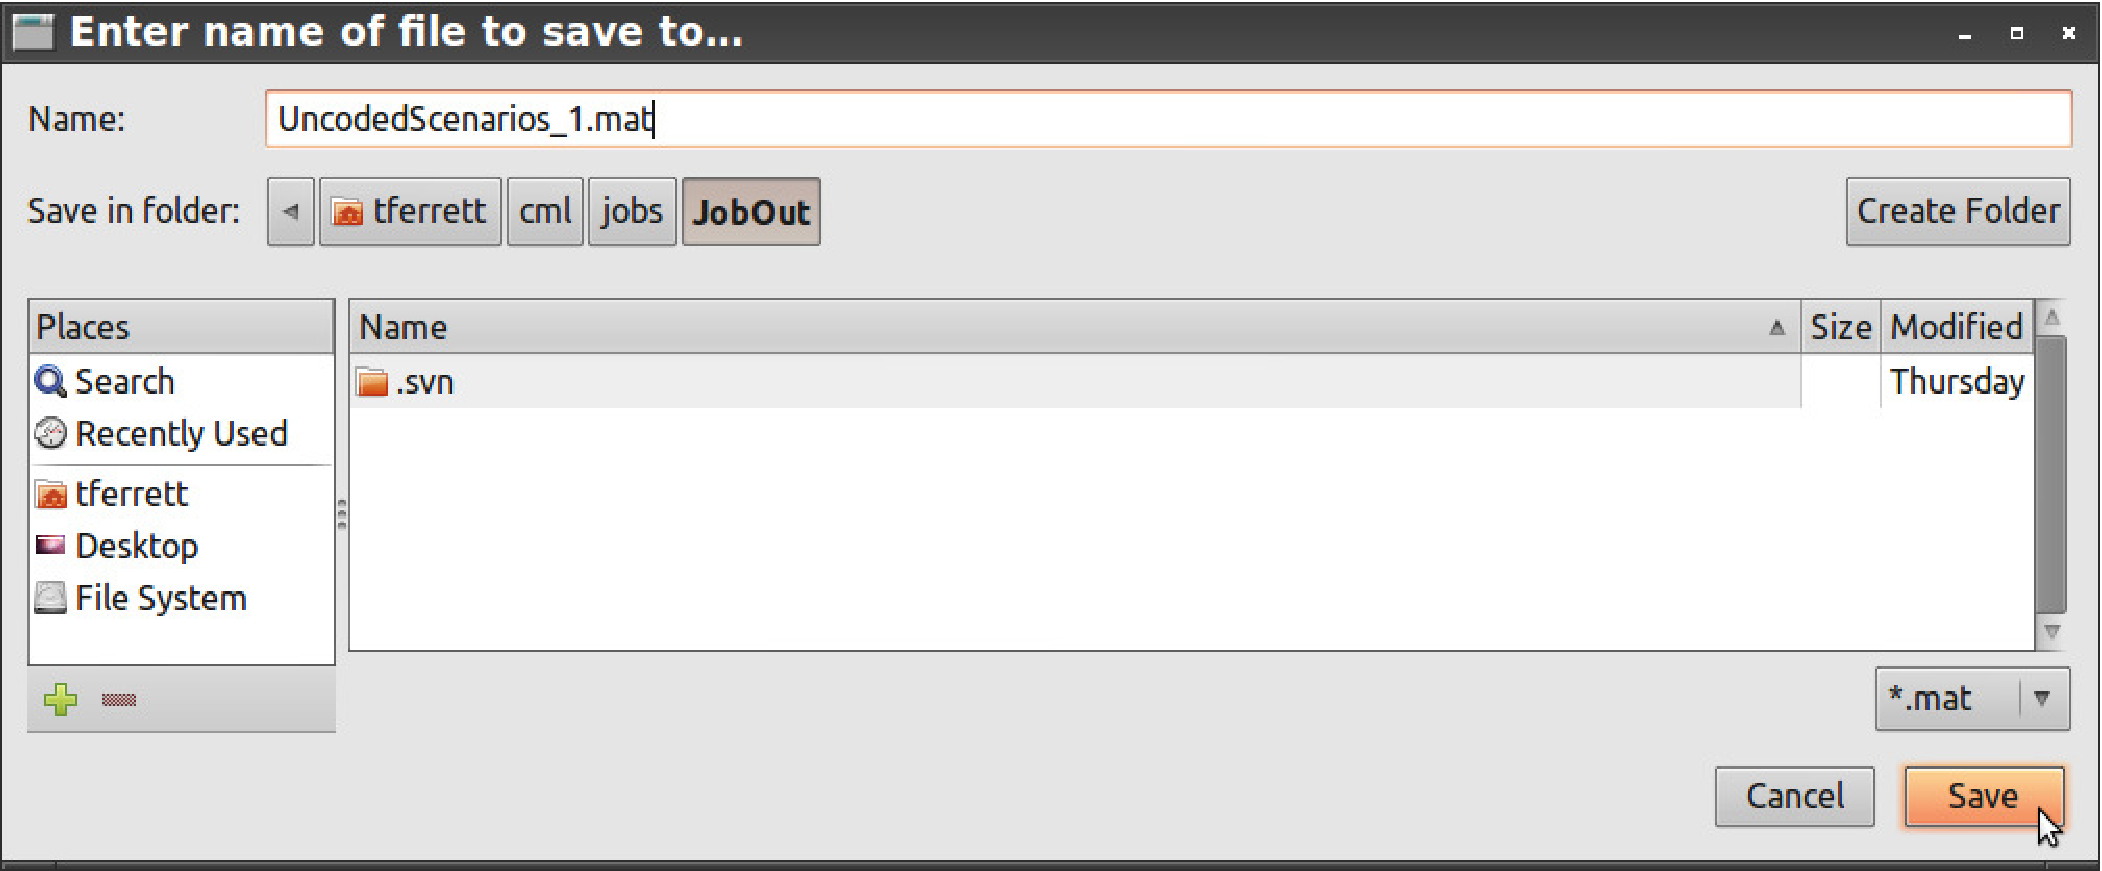
\includegraphics[width=0.9\textwidth]{wcrlctc_jobout}
  \end{figure}

\end{frame}




% cmlwebretrieve
\begin{frame}
  \frametitle{Job File Conversion and Result Plotting}

  The completed job file must be converted to a CML output file appropriate for plotting.
  \begin{itemize}
  \item Execute the function 'CmlWebRetrieve' to convert the job file to a CML output file as shown in the figure.
  \item The results of simulation may now be plotted as shown.
  \end{itemize}

  \centering
  \begin{figure}
    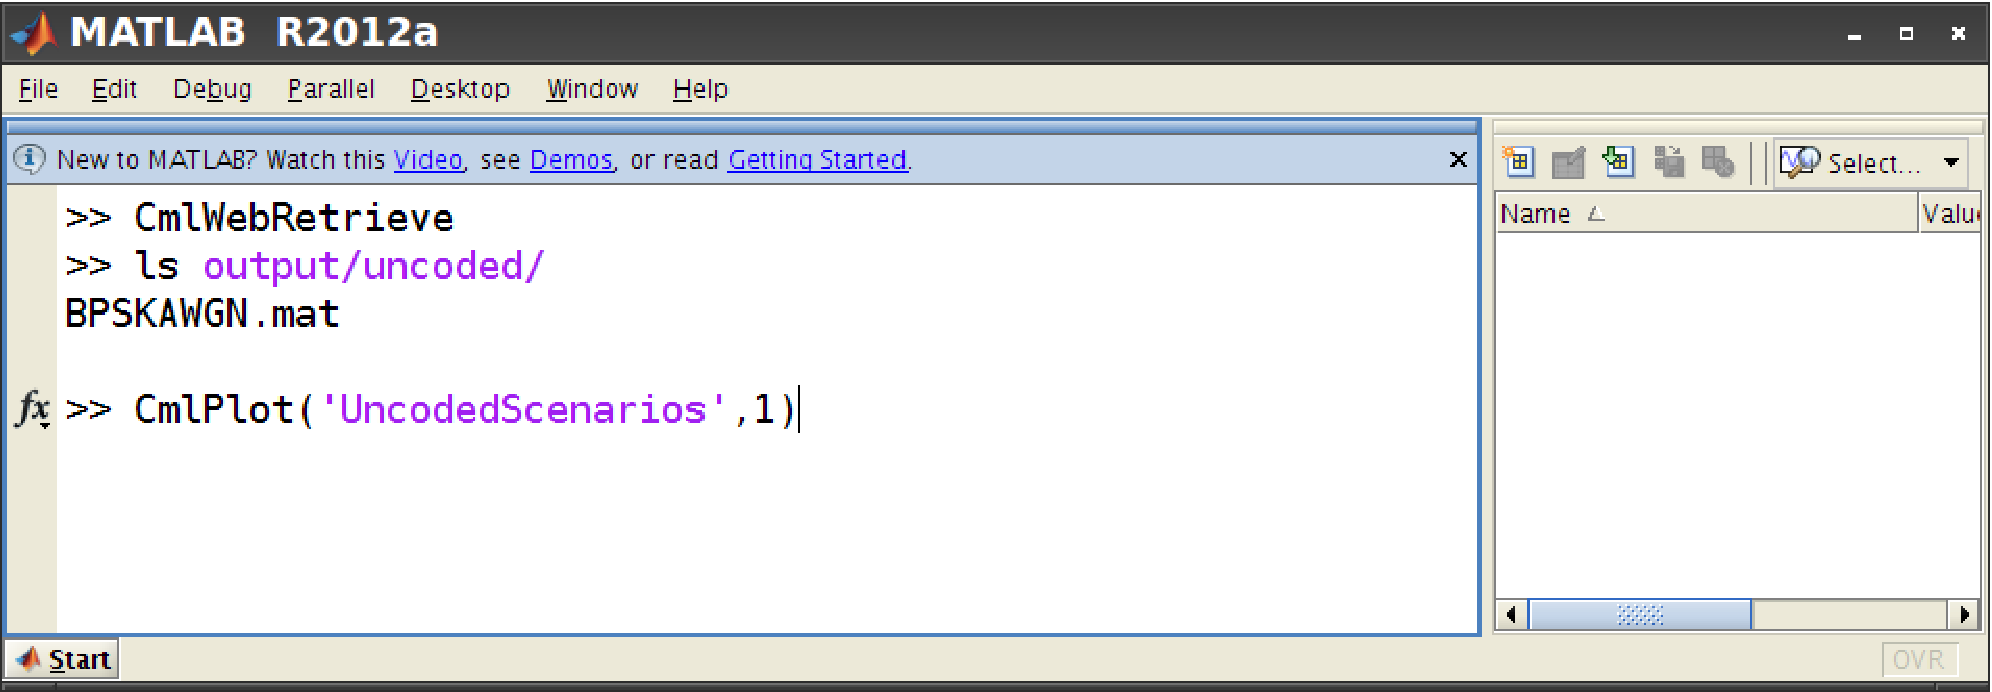
\includegraphics[width=0.9\textwidth]{cml_webretrieve}
  \end{figure}

\end{frame}



% plotted results
\begin{frame}

  \centering
  \begin{figure}
    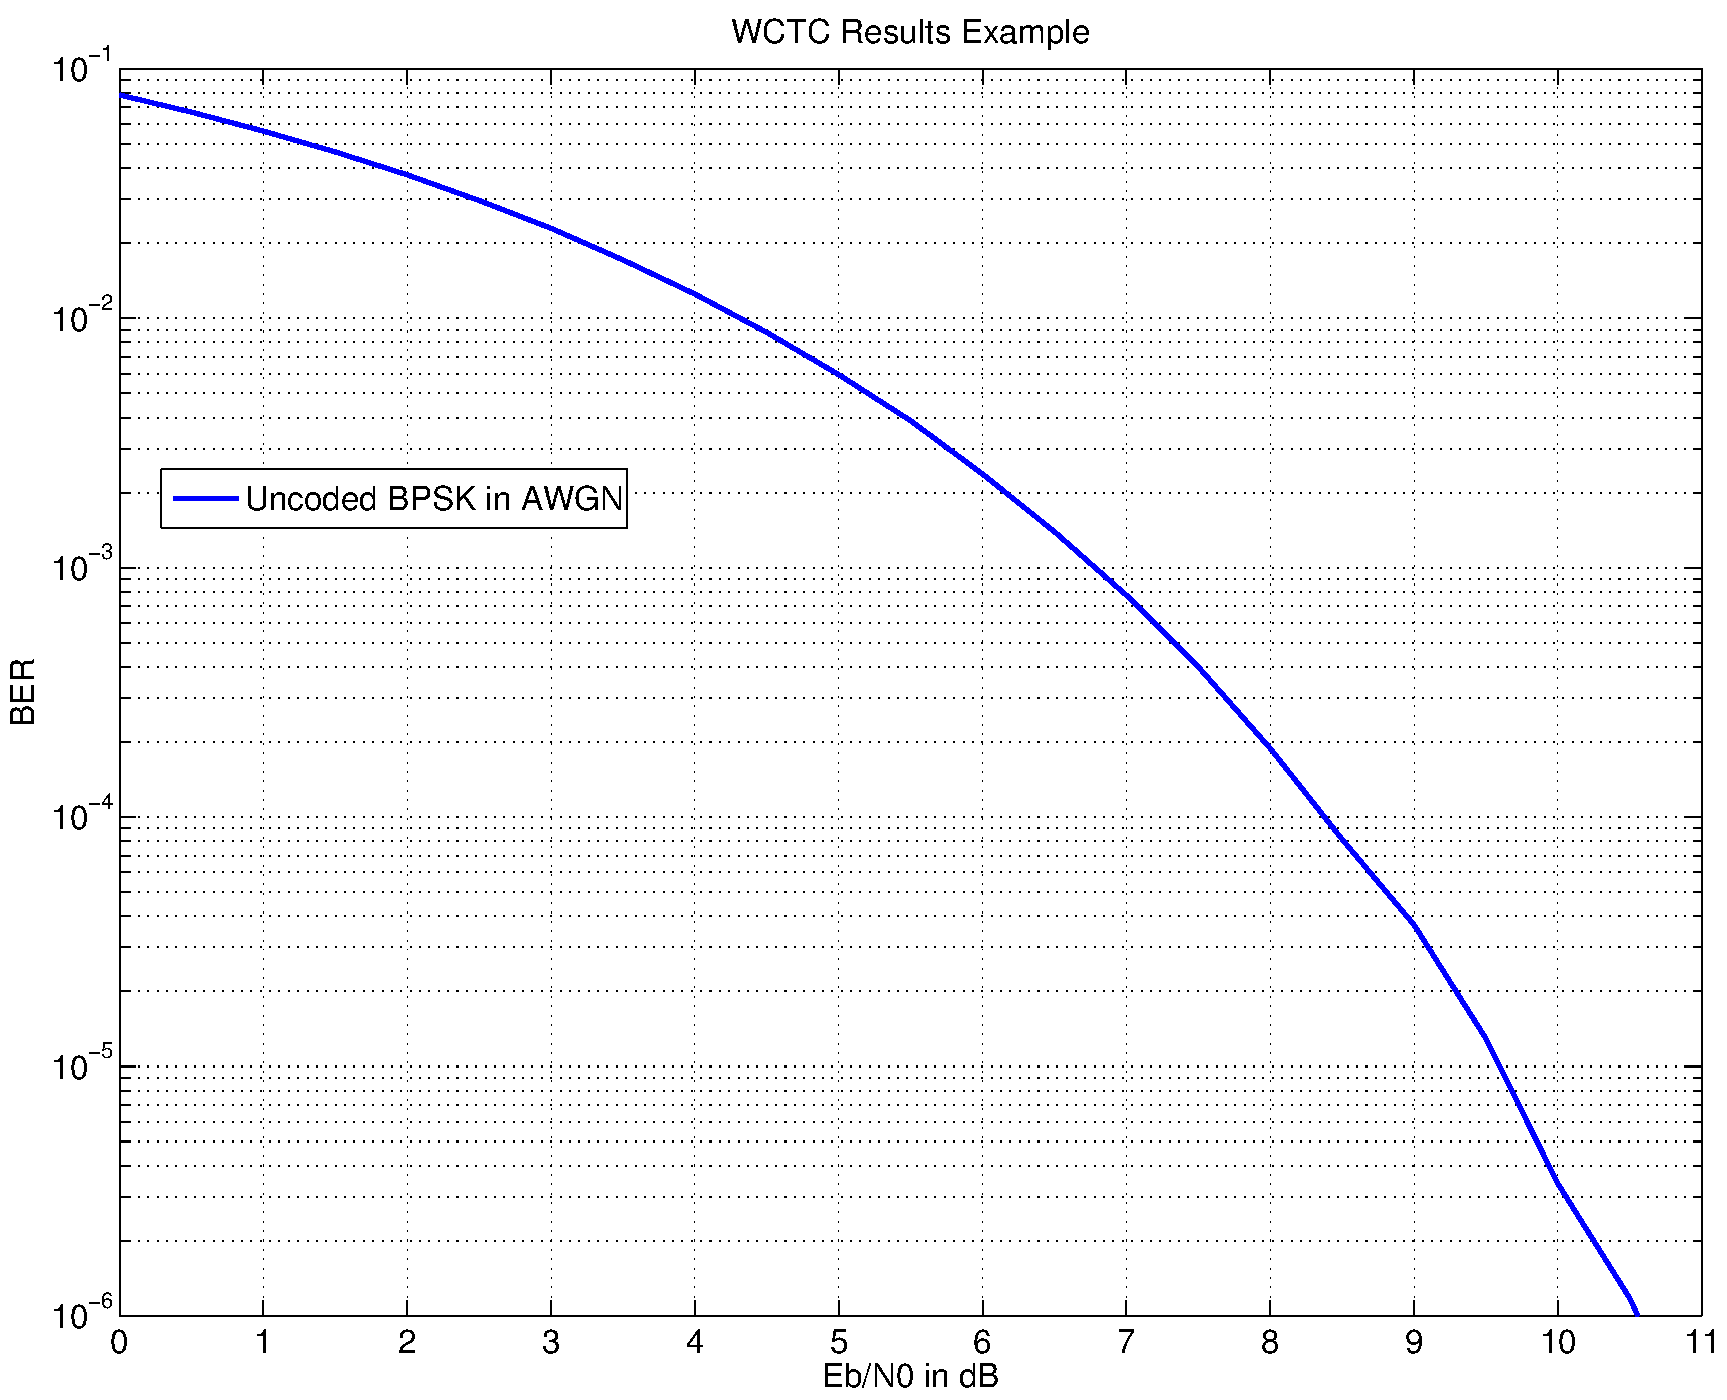
\includegraphics[width=0.8\textwidth]{cml_res}
  \end{figure}

\end{frame}







\section{Job Submission Summary}
\begin{frame}
\frametitle{Steps to Submitting a Job}

\begin{enumerate}
\item Create a WCTC account at \url{http://wctc.csee.wvu.edu}

\item Download and install CML from \url{http://code.google.com/p/iscml/wiki/cml}

\item Select a CML error-rate scenario and record to simulate and create a job file using
\\ $>>$ CmlWebSubmit(scenario, record)
\vspace{3mm}
\\ The job file is located in $<$CMLROOT$>$/jobs/JobIn/$<$scenario$>$\_$<$record$>$.mat

\item Log in to the WCTC web interface and upload the job file.

\item Once the job is completed, download the job results file to \\
$<$CMLROOT$>$/jobs/JobOut/$<$scenario$>$\_$<$record$>$.mat

\item Convert the job results file to a CML output file and plot
\\ $>>$ CmlWebRetrieve
\\ $>>$ CmlPlot(scenario, record)
\end{enumerate}

\end{frame}

%%%%%%%%%%%%%%%%%%%%%%%%%%%%%%%%%%% 




\end{document}





